\frame{
backup slides from here on
}

\frame{
	\frametitle{Synthetic radiograms}
	
	\begin{textblock}{0.9}(0.03,0.05)
		\centering
		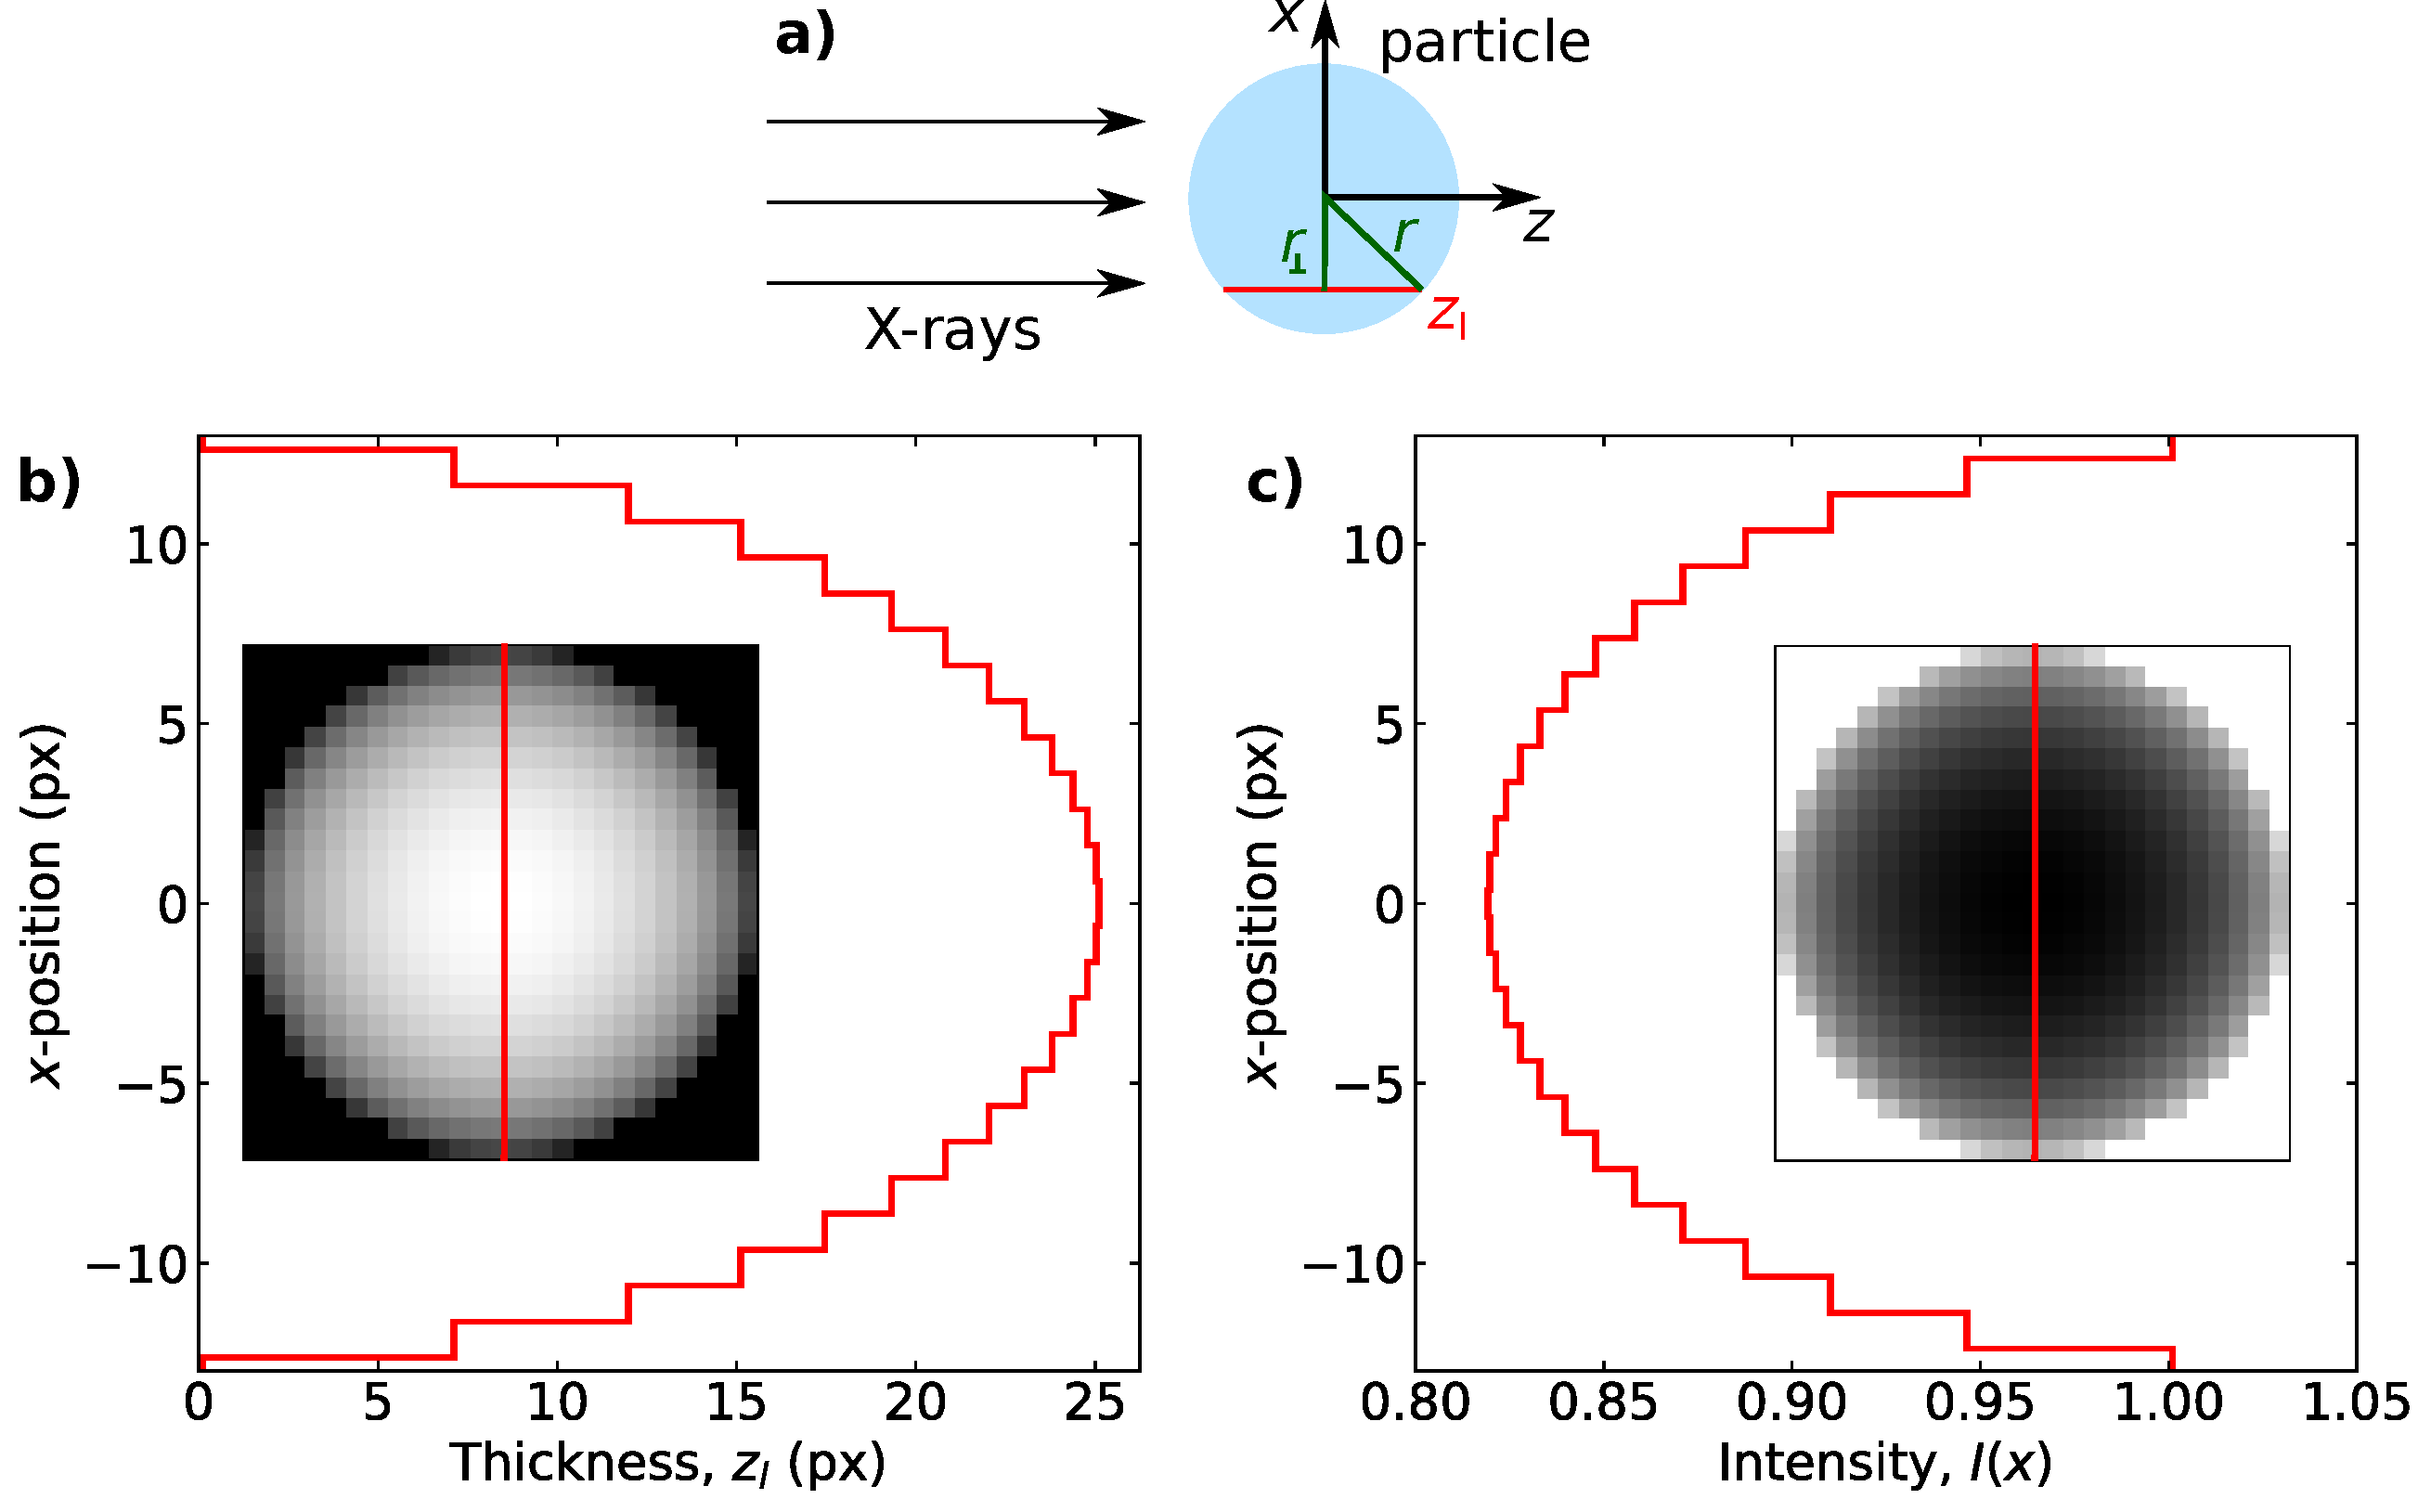
\includegraphics[width=0.6\textwidth]{Sources/X-DFA/particle_mask_construction.pdf}
	\end{textblock}
	
	\begin{textblock}{0.9}(0.05,0.8)
		\centering
		Beer-Lambert\\
		$I(z_l) = I_0 \exp(-\mu z)$
	\end{textblock}
	
	\begin{textblock}{0.2}(0.03,0.6)
		\visible<2->{
			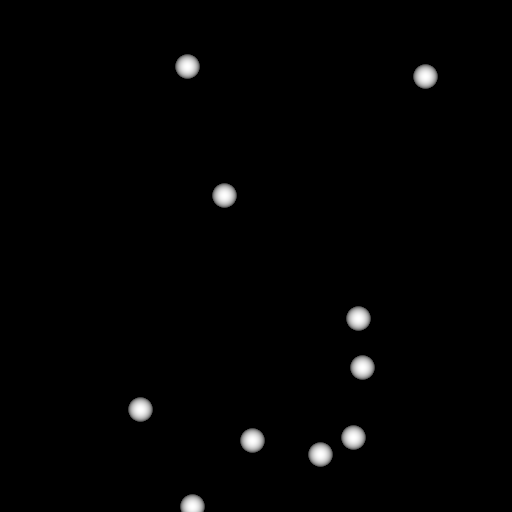
\includegraphics[width=\textwidth]{Sources/X-DFA/thicknessMap_nPart10.png}}
	\end{textblock}
	
	\begin{textblock}{0.2}(0.77,0.6)
		\visible<2->{
			\frame{
				
\includegraphics[width=\textwidth]{Sources/X-DFA/fake_img_nPart10.png}
		}}
	\end{textblock}
}

\frame{
	\frametitle{Linear space invariant imaging}
	\begin{textblock}{0.5}(0.0,0.15)
		\visible<1->{
			\centering
			Image correlation function
			\[
			g(\mathbf{q}, \tau) = \frac
			{\langle I^*(\mathbf{q},t) I(\mathbf{q},t+\tau) \rangle_t}
			{\langle |I(\mathbf{q},t)|^2 \rangle_t}
			\]
		}
	\end{textblock}
	
	
	
	\begin{textblock}{0.5}(0.5,0.15)
		\visible<2->{
			\centering
			Intermediate scattering function
			\[
			f(\mathbf{q},\tau) = \frac
			{\langle \rho^*(\mathbf{q},t) \rho(\mathbf{q},t+\tau) \rangle_t}
			{\langle |\rho(\mathbf{q},t)|^2 \rangle_t}
			\]}
	\end{textblock}
	
	\begin{textblock}{0.9}(0.05,0.42)
		\visible<2->{	
			Linear space-invariant imaging:
			\begin{align}
			I(\mathbf{r},t) = I_0 + \int \mathsf{d}\mathbf{r}' \ \mathsf{d}z'
			T(\mathbf{r}-\mathbf{r}',-z') c(\mathbf{r}',z',t)
			\nonumber
			\end{align}
		}
	\end{textblock}
	
	
	\begin{textblock}{0.9}(0.05,0.6)
		\visible<2->{
			\centering
			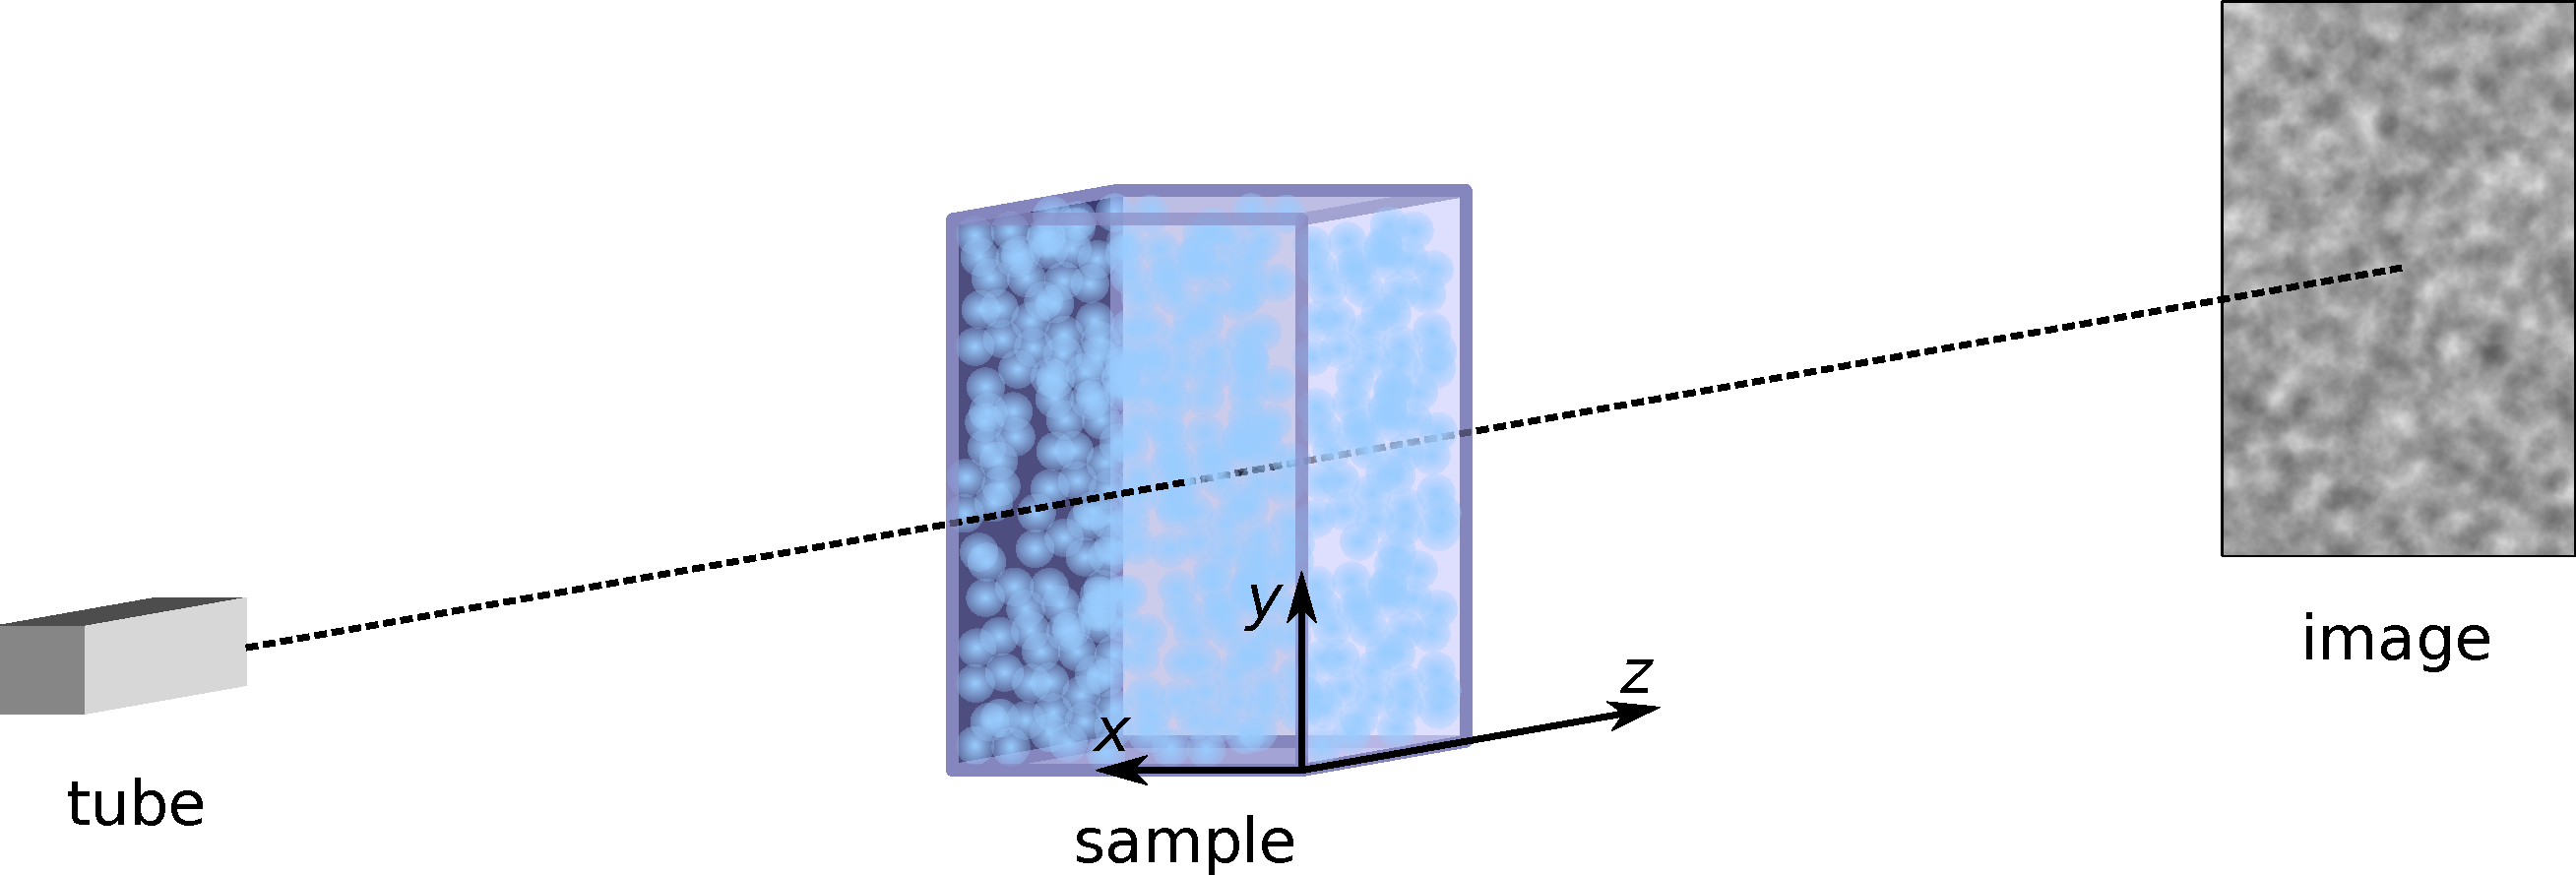
\includegraphics[width=0.7\textwidth]
			{Sources/X-DFA/image_transfer_function1.pdf}
		}
	\end{textblock}
	
}